\section{Methodology}
\begin{enumerate}
	\item Motivation
	\par In practice, we may meet some hard integrations which is really hard to solve. For example, in one of my working papers, we have this integrand
		\begin{equation*}
			CARL = (1 - \Phi(\frac{\Phi^{-1}(u)}{\sqrt{k}} + \frac{c}{c_4}\sqrt{\frac{F^{-1}_{\chi^2_{k-1}(v)}}{k-1}}) + \Phi(\frac{\Phi^{-1}(u)}{\sqrt{k}} - \frac{c}{c_4}\sqrt{\frac{F^{-1}_{\chi^2_{k-1}(v)}}{k-1}}))^{-1}, 0<u<1, 0<v<1
		\end{equation*}
		where $k$, $c$ and $c_4$ are constants. $\Phi$ is the c.d.f. of the standard normal distribution. $\Phi^{-1}$ is the quantile function the standard normal distribution. $F^{-1}_{\chi^2_{k-1}}$ is the quantile function of $\chi^2$ with $k-1$ degrees of freedom. 
		\par The analytical solution probably is desperate, but we can use other methods to obtain the numerical solution. This handout will show a way to solve integrations numerically.
	
	\item Example. $Y = |X|$ where $X \sim N(0, 1)$. Find out $E(Y)$
		\begin{enumerate}
			\item Method 1: Direct Integration (By hand)
				\par As we know, the p.d.f. of $Y$
				\begin{equation*}
					f_Y(y) = 2\phi(y), y \ge 0
				\end{equation*}
				where $\phi$ is the p.d.f. of the standard normal distribution. The expectation
				\begin{equation*}
					\begin{split}
						E(Y) &= \int_{0}^{\infty} 2y\phi(y) dy \\
						& = \frac{1}{\sqrt{2\pi}}\int_{0}^{\infty} 2y e^{-\frac{1}{2}y^2}dy \\
						& = \frac{2}{\sqrt{2\pi}}\int_{0}^{\infty} \frac{1}{2} e^{-\frac{1}{2}y^2}dy^2 \\
						& = \sqrt{\frac{2}{\pi}} \approx 0.7979
					\end{split}
				\end{equation*}
			\item Method 2: Direct Integration (In R)
				\begin{itemize}
					\item R code
					\begin{verbatim}
						# define the p.d.f. of Y
						Y.pdf <- function(y) 2 * dnorm(y)
						
						# define the integrand of the expecation of Y
						E.Y <- function(y) y * Y.pdf(y)
						
						# Integrate the integrand
						integrate(E.Y, lower = 0, upper = Inf)
						# Result: 0.7978846
					\end{verbatim}
				\end{itemize}
			\item Monte Carlo Method
			\par Suppose $X$ is a random variable with a p.d.f. $f$ and a c.d.f. $F$ over a domain $D$. Also, we have a sample $X_s = \{x_1, x_2, ..., x_n\}$ from $X$ with $n$ observations.
			\begin{equation*}
			E(X) = \int_{D}xf(x)dx \approx \bar{X} = \frac{1}{n} \sum_{i = 1}^{n}x_i
			\end{equation*}
			Besides, because of Central Limit Theorem, $\bar{X}$ asymptotically follows $N(\mu, \frac{\sigma^2}{n})$ where $\mu = E(X)$ is the mean of $X$ and $\sigma^2$ is the variance of $X$. So, when $n \rightarrow \infty$, $\bar{X} \rightarrow E(X)$. Hence, intuitively, the result is more precise with a larger sample size.
			\begin{enumerate}
				\item Method 3: Monte Carlo Method with Transformation 1
				\par Because 
				\begin{equation*}
				E(Y) = E(|X|) = \int_{-\infty}^{\infty}|x| \phi(x)dx \approx \frac{1}{n}\sum_{i = 1}^{n} |x_i|
				\end{equation*}
				where $n$ is the number of simulation and $X_s = \{ x_1, ..., x_n\}$ is a sample from $N(0, 1)$.
				\begin{itemize}
					\item R code
					\begin{verbatim}
					# set seed to make this process repeatable
					set.seed(12345)
					
					# set the number of simulation
					n <- 1000
					
					# simulate a sample from the standard 
					# normal distribution
					X.s <- rnorm(n)
					
					# calculate the mean of the absoluate values
					mean(abs(X.s))
					# Result: 0.7944
					\end{verbatim}
				\end{itemize}
				\item Method 4: Monte Carlo Method with Transformation 2
				\par Because $exp(1)$ has a same domain as $Y$, 
				\begin{equation*}
				E(Y) = \int_{0}^{\infty}yf_Y(y)dy = \int_{0}^{\infty}\frac{yf_y(y)}{e^{-y}}e^{-y}dy = E(\frac{yf_Y(y)}{e^{-y}}) \approx \frac{1}{n}\sum_{i=1}^{n}\frac{y_if_Y(y_i)}{e^{-y_i}}
				\end{equation*}
				where $n$ is the number of simulation and $Y_s = \{y_1, ..., y_n\}$ is a sample from $exp(1)$.
				\begin{itemize}
					\item R code
					\begin{verbatim}
					# set seed to make this process repeatable
					set.seed(12345)
					
					# set the number of simulation
					n <- 1000
					
					# define the p.d.f. of Y
					Y.pdf <- function(y) 2 * dnorm(y)
					
					# simulate a sample from the standard 
					# normal distribution
					Y.s <- rexp(n)
					
					# calculate the mean of the absoluate values
					mean(Y.s * Y.pdf(Y.s) / dexp(Y.s))
					# Result: 0.7729
					\end{verbatim}
				\end{itemize}
			\end{enumerate}
		\end{enumerate}
	\item Summary
		\begin{enumerate}
			\item Comparison of these methods
			\begin{center}
				\begin{tabular}{c | c | c | c | c}
					Methods & Method 1 & Method 2 & Method 3* & Method 4* \\
					\hline
					Results & 0.7979 & 0.7979 & 0.7944 & 0.7729
				\end{tabular}
			\end{center}
			* Method 3 and Method 4 have 1000 simulations.
			\item Steps of Monte Carlo Method
			\begin{enumerate}
				\item Check the domain
				\item Simulate an appropriate sample over the domain 
				\item Calculate the mean via an appropriate transformation
			\end{enumerate}
		\end{enumerate}
	\item Practice: suppose $Y = X^{-1}$, where $X \sim \chi^2(10)$. Use Monte Carlo Method to find $E(Y)$.
	\par Hint: You need to show the analytical part and the coding part in R, separately. Also, you may need to use $rchisq$ and $help(rchisq)$ in R
\end{enumerate}

\newpage
\section{Application}
\begin{enumerate}
	\item Data description\cite{civ17}
	\par This data comes from the Vancouver Open Data Catalogue. It has 530,652 records regarding to different types of crimes between Jan 01, 2003 and July 13, 2017. The original data set contains coordinates in UTM Zone 10 with Latitude and Longitude. 
	\item Suppose our target is to predict the monthly frequency of the type of crimes "Break and Enter Commercial" in the future and we are not very interested in the exact locations of crimes. The frequency during the period between Jan 01, 2003 and July 13, 2017 can be showed as the following plot:
	\begin{center}
		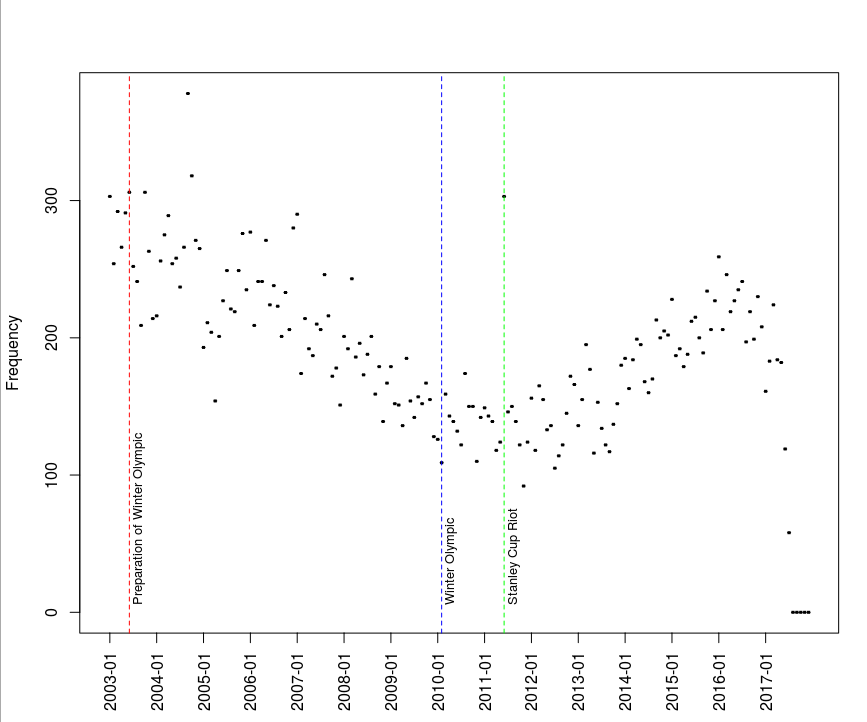
\includegraphics[scale=0.5]{/home/yuhuiyao/Documents/Github/R-handout/MCandApp/Handout/plot1.png}
	\end{center}
	where on July 2, 2003, Vancouver won the bid to host the Winter Olympic (the vertical red dashed line). The game was hosted from February 12 to 28, 2010 (the vertical blue dashed line). So I called the period between July 2, 2003 and February, 28, 2010 as the preparation of Winter Olympic. Also, on June 15, 2011, there was a riot, 2011 Vancouver Stanley Cup riot (the vertical green dashed line). It is obvious for us to observe that the frequency has a convex shape and one of possible reasons causing this phenomenon is the Winter Olympic. 
	\par Intuitively, I will guess the frequency of crimes are increasing until reaching the situation before the preparation of Winter Olympic. Hence, I will use the fraction of the data before July 2003, as my training data, to predict the frequency after 2017.
	\item
	\par Suppose $X = \{303, 254, 292, 266, 291, 306\}$ is from my training data and this data follows a Poisson distribution with parameter $\lambda$. Find out the 2.5\% and 97.5\% quantile. The p.d.f. of $X$
	\begin{equation*}
		f_X(x) = \frac{\lambda^{x}e^{-\lambda}}{x!} , x = 0, 1, 2, ...
	\end{equation*}
	By m.l.e, $\hat{\lambda} = \bar{X} = 285.3333$, so the 2.5\% and 97.5\% quantile
	\begin{equation*}
		\begin{cases}
			0.025 = \sum_{t = 1}^{q_{0.025}}\frac{\lambda^{t}e^{-\lambda}}{t!} \\
			0.975 = \sum_{t = 1}^{q_{0.975}}\frac{\lambda^{t}e^{-\lambda}}{t!} 
		\end{cases} \Rightarrow \begin{cases}
			q_{0.025} = 253 \\
			q_{0.975} = 319
		\end{cases}
	\end{equation*}
	They can be showed on the plot
	\begin{center}
		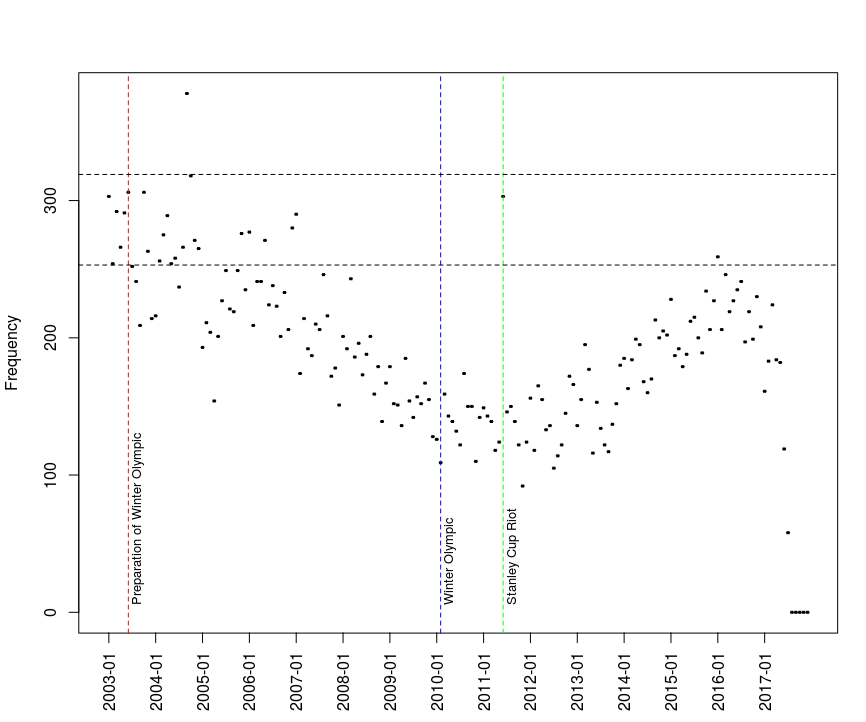
\includegraphics[scale=0.4]{/home/yuhuiyao/Documents/Github/R-handout/MCandApp/Handout/plot2.png}
	\end{center}
	where the upper horizontal dashed line is the 97.5\% quantile, 319 and the lower horizontal dashed line is the 2.5\% quantile, 253.
	\item Because $X$ is a sample, $\hat{\lambda} = \bar{X}$ shall have its own distribution. Suppose $\hat{\lambda} \sim gamma(\alpha= 1125.168, \beta = 0.2536)$. Find out the 2.5\% and 97.5\% quantile.
	\par The p.d.f. of $X$ given $\hat{\lambda}$
	\begin{equation*}
			f_{X|\hat{\lambda}}(x) = \frac{\lambda^{x}e^{-\lambda}}{x!}
	\end{equation*}
	\par And the p.d.f. of $\hat{\lambda}$
	\begin{equation*}
		f_{\hat{\lambda}}(\lambda) = \frac{1}{\Gamma(\alpha)\beta^{\alpha}}\lambda^{\alpha - 1}e^{-\frac{\lambda}{\beta}}d\lambda, \lambda > 0
	\end{equation*}
	Then
	\begin{equation*}
		\begin{split}
			P(X \le x) &= \int_{0}^{\infty}P(X < x | \hat{\lambda} = \lambda)f_{\hat{\lambda}}(\lambda) d \lambda \\
			& = \int_{0}^{\infty}(\sum_{t = 1}^{x}\frac{\lambda^{t}e^{-\lambda}}{t!})(\frac{1}{\Gamma(\alpha)\beta^{\alpha}}\lambda^{\alpha - 1}e^{-\frac{\lambda}{\beta}}) d \lambda
		\end{split}
	\end{equation*}
	So, the 2.5\% and 97.5\% quantile
	\begin{equation*}
		\begin{cases}
		0.025 = \int_{0}^{\infty}(\sum_{t = 1}^{q_{0.025}}\frac{\lambda^{t}e^{-\lambda}}{t!})(\frac{1}{\Gamma(\alpha)\beta^{\alpha}}\lambda^{\alpha - 1}e^{-\frac{\lambda}{\beta}}) d \lambda \\
		0.975 = \int_{0}^{\infty}(\sum_{t = 1}^{q_{0.975}}\frac{\lambda^{t}e^{-\lambda}}{t!})(\frac{1}{\Gamma(\alpha)\beta^{\alpha}}\lambda^{\alpha - 1}e^{-\frac{\lambda}{\beta}}) d \lambda
		\end{cases}
	\end{equation*}
	The analytical solution is complicated, but it is relatively easy if we use numerical methods. By Monte Carlo Method,
	\begin{equation*}
		P(X \le x) = \int_{0}^{\infty}(\sum_{t = 1}^{x}\frac{\lambda^{t}e^{-\lambda}}{t!})(\frac{1}{\Gamma(\alpha)\beta^{\alpha}}\lambda^{\alpha - 1}e^{-\frac{\lambda}{\beta}}) d \lambda = E(\sum_{t = 1}^{x}\frac{\lambda^{t}e^{-\lambda}}{t!})) \approxeq \frac{1}{n} \sum_{i = 1}^{n} \sum_{t = 1}^{x}\frac{\lambda_i^{t}e^{-\lambda_i}}{t!}
	\end{equation*}
	where $\lambda_s = \{\lambda_1,...,\lambda_n \}$ is a sample following $gamma(\alpha= 1125.168, \beta = 0.2536)$. Also, the equation can be expressed as the following (the root searching form)
	\begin{equation*}
		P(X \le x) - \frac{1}{n} \sum_{i = 1}^{n} \sum_{t = 1}^{x}\frac{\lambda_i^{t}e^{-\lambda_i}}{t!} = 0
	\end{equation*}
	where $P(X \le q_{0.025}) = 0.025$ and $P(X \le  q_{0.975}) = 0.975$. The quantiles $q_{0.025}$ and $q_{0.975}$ are roots of the equation. 
	\begin{center}
		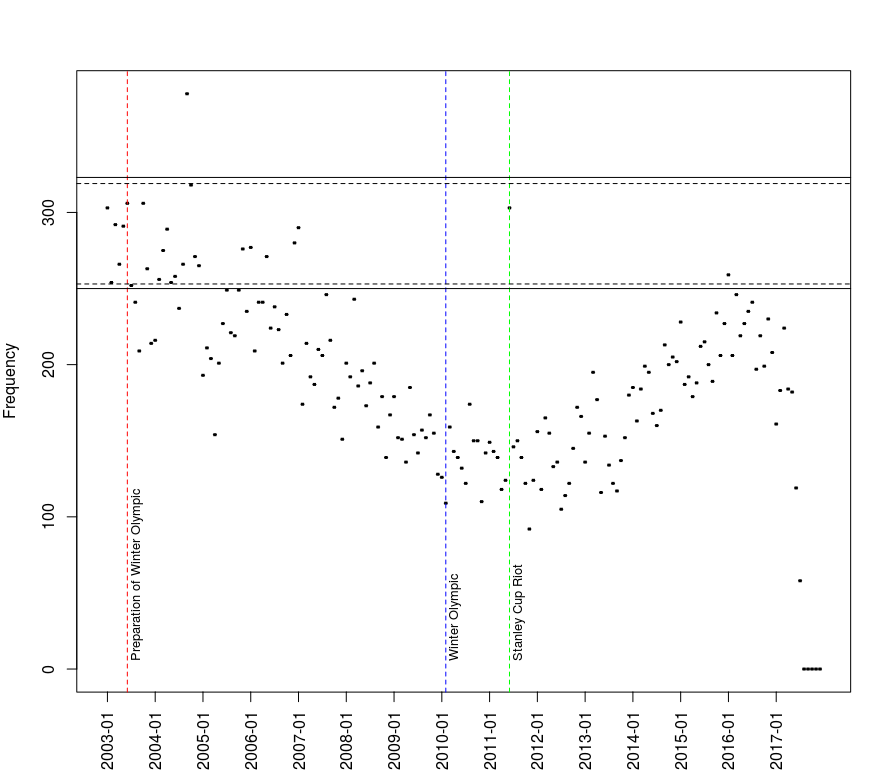
\includegraphics[scale=0.4]{/home/yuhuiyao/Documents/Github/R-handout/MCandApp/Handout/plot3.png}
	\end{center}
	where the upper horizontal solid line is the 97.5\% quantile, 323 and the lower horizontal solid line is the 2.5\% quantile, 249.
	\item R code for the whole process
	\begin{verbatim}
		#################################################
		# describe BEC during the period
		#################################################
		# load the new data
		addr <- paste('https://raw.githubusercontent.com/bolus123', 
		'/R-handout/master/MCandApp/BEC.csv', sep = '')
		BEC.monthly.freq <- read.csv(file = addr)[, -1]
		
		# add a new column combining YEAR with MONTH
		BEC.monthly.freq <- cbind(BEC.monthly.freq, 
		paste(BEC.monthly.freq$YEAR, 
		substr(
		as.character(
		as.numeric(
		BEC.monthly.freq$MONTH) + 
		100), 2, 3)
		, sep = '-'))
		
		# build a basic scatter frequency plot 
		# during the period
		plot(BEC.monthly.freq[, 5], BEC.monthly.freq[, 4], 
		xaxt="n", ylab = 'Frequency')
		# define the tick of x-axis
		labs <- sort(BEC.monthly.freq[, 5])[rep(c(T, F, F, 
		F, F, F, F, F, F, F, F, F), 15)]
		for (i in 1:15){
		
		axis(1, at = (12 * (i - 1) + 1), 
		labels = labs[i], las = 2)
		
		}
		
		# specify special months
		prepare.Winter.Olympic <- BEC.monthly.freq[, 5] == '2003-06'
		Winter.Olympic <- BEC.monthly.freq[, 5] == '2010-02'
		Stanley.Cup.riot <- BEC.monthly.freq[, 5] == '2011-06'
		
		# show Preparation of Winter Olympic on the plot
		abline(v = BEC.monthly.freq[prepare.Winter.Olympic, 5], 
		col = 'red', lty = 2)
		text(BEC.monthly.freq[prepare.Winter.Olympic, 5], 5, 
		'Preparation of Winter Olympic', pos = 4, 
		srt = 90, cex = 0.8)
		
		# show Winter Olympic on the plot 
		abline(v = BEC.monthly.freq[Winter.Olympic, 5], 
		col = 'blue', lty = 2)
		text(BEC.monthly.freq[Winter.Olympic, 5], 5, 
		'Winter Olympic', pos = 4, srt = 90, cex = 0.8)
		
		# show Stanley Cup Riot on the plot 
		abline(v = BEC.monthly.freq[Stanley.Cup.riot, 5], 
		col = 'green', lty = 2)
		text(BEC.monthly.freq[Stanley.Cup.riot, 5], 5, 
		'Stanley Cup Riot', pos = 4, srt = 90, cex = 0.8)
		
		# set the maximun date of the training data
		x1.max.date <- which(
		BEC.monthly.freq[
		order(BEC.monthly.freq[, 5]), 5] == '2003-06')
		
		# cut it off from the original data
		x1 <- BEC.monthly.freq[
		order(BEC.monthly.freq[, 5]), 4][1:x1.max.date]
		
		# fit a poisson model for the training data
		lambda1 <- mean(x1)
		
		# show the 2.5% and 97.5 quantiles on the plot
		abline(h = qpois(0.975, lambda1), lty = 2)
		abline(h = qpois(0.025, lambda1), lty = 2)
		
		#################################################
		# find the gamma distribution for lambda 
		# by the nonparametric bootstrap
		#################################################
		set.seed(12345)
		
		# the number of times for bootstrapping
		n <- 100000
		# set a vector to carry the means
		xs.means <- rep(NA, n)
		
		for (i in 1:n){
		
		# resample from the training data
		xs <- sample(x1, 5, replace = T)
		
		# calculate their means
		xs.means[i] <- mean(xs)
		
		}
		
		# calculate the grand mean
		mu <- mean(xs.means)
		# calculate the grand variance
		sigma2 <- var(xs.means)
		
		# fit a gamma model by the method of moment
		alpha <- mu^2 / sigma2
		beta <- sigma2 / mu
		
		# check the gamma distribution
		#x <- 1:1000 
		#plot(x, dgamma(x, alpha, 1/beta), type = 'l')
		
		#################################################
		# fit a new poisson model 
		# with parameter lambda 
		# which is a random variable
		#################################################
		# set a seed make this process repeatable
		set.seed(12345)
		
		# define a user-defined function
		# p is P(X <= x)
		# alpha is the alpha for gamma(alpha, beta)
		# beta is the beta for gamma(alpha, beta)
		# interval is the range of searching the quantile
		# rnum is the number of simulations
		X.quantile <- function(p, alpha, beta, 
		interval = c(100, 500), rnum = 10000){
		
		root.finding <- function(x, p, lambda){
		
		# The root searching form
		p - mean(ppois(x, lambda))
		
		}
		
		# simulate a sample from gamma distribution
		lambda <- rgamma(rnum, alpha, scale = beta)
		
		# search the root by the bisection method
		uniroot(root.finding, interval = interval, 
		p = p, lambda = lambda)$root
		
		
		}
		
		# calcualte the 2.5% quantile
		q0025 <- X.quantile(p = 0.025, 
		alpha = alpha, beta = beta)
		# calcualte the 97.5% quantile
		q0975 <- X.quantile(p = 0.975, alpha = alpha, beta = beta)
		
		# add horizontal lines on the plot
		abline(h = q0025)
		abline(h = q0975)
	\end{verbatim}
\end{enumerate}